\documentclass[12pt]{article}
%
% % Insert style guide
\usepackage{my_thesis}

% Specifiy the location of images to be used
\graphicspath{{figures/}}

%

\begin{document}
\title{\textsc{Surface waves extraction of a conductive sheet embedded in a multilayer environment}}

\date{\footnote{Last Modified: \currenttime, \today.}}

% Create title page
\maketitle

%\chapter{\uppercase{Surface waves extraction using transmission line Green functions in a multilayer environment with a 2D sheet}}



% \section{Abstract}

In this chapter, we compute the dispersion diagrams of an infinitesimally thin conductive that lies embedded in a stack of semiconductors. The possibility of wave propagation along the sheet is investigated by searching for poles of an equivalent transmission line Green function determined by the multilayer structure. A numerical root-finding routine is presented that permits complex-valued solutions and avoids singularities in the complex plane.

\section{Theory}


\subsection{Derivation of Transmission line Green Function}

We follow the well-established approach of field computation for planar multilayered media \cite{michalski1997multilayered, michalski2005}, in which an equivalent transmission line network is set up for the structure. As shown in Fig. \ref{fig:TL_equivalent}a, it is assumed that the structure is unbounded in the lateral direction. The electric and magnetic fields are given by the Maxwell's equations,
\begin{subequations}
  \begin{align}
    \del\x{\v E} ={}& -j \O \u \v{H},
    \label{eq:E}\\
    \del\x{\v H} ={}& j \O \E \v{E} + \v{J}.
    \label{eq:H}
  \end{align}
  \label{eq:MaxE}%
\end{subequations}
%
For boundary-value problems displaying symmetry along the $z$ direction, it is desirable to decompose the $\v{\del}$ operator into two components, one $d/dz$ and the other a transverse (to z) operator, $\v{\del_t}$ \cite[p. 64]{felsen1994}. By taking the Fourier transform,
%
\begin{equation}
    \mathcal{F}[f(\v{r})] \equiv \ti{f}(\v{k_{\p}},z) = \infint \infint
    f(\v{r}) \e^{-\j \v{k_{\p}} \cdot \v{\p}} \diff{x} \diff{y}
    \label{eq:Fourier}
\end{equation}
%
the field computation is simplified by switching to the spectral frequency domain $\v {k_{\p}}$, which reduces the vector differential operator, $\v{\del}$ to $-\j k_x \v{\^{x}} - \j k_y \v{\^{y}} + d/dz\, \v{\^{z}}$. In \eqref{eq:Fourier}, the cylindrical coordinates are expressed as,
%
\begin{equation}
  \v{\p} = x\v{\^{x}} + y\v{\^{y}}, \quad \text{and} \quad
  \v{k_{\p}} = k_x\v{\^{x}} + k_y\v{\^{y}},
\end{equation}
%
and the notation $\sim$ above the terms indicates the Fourier transform with respect to the transverse coordinates and from here on, will be used to denote the spectral domain quantities.

As stated earlier, it is advantageous to separate the fields in transverse and longitudinal coordinates since, as we shall shortly see, the longitudinal part of the field can be completely expressed in terms of the transverse component. Appling the Fourier transform \eqref{eq:Fourier} on the Maxwell's equations \eqref{eq:MaxE}, we obtain:
%
\begin{subequations}
  \begin{align}
    \left(-\j \v{k_{\p}} + \v{\^{z}} \dv{}{z} \right)\x (\v{\ti{E}_t} + \v{\ti{E}_z})  ={}& -\j \O \u (\v{\ti{H}_t} + \v{\ti{H}_z}),
    \label{eq:FT_E}\\
    \left(-\j \v{k_{\p}} + \v{\^{z}} \dv{}{z} \right)\x (\v{\ti{H}_t} + \v{\ti{H}_z})  ={}& \j \O \E (\v{\ti{E}_t} + \v{\ti{E}_z}) -
    (\v{\ti{J}_t} + \v{\ti{J}_z}).
    \label{eq:FT_H}
  \end{align}
  \label{eq:FT_EH}%
\end{subequations}
%
The transverse and longitudinal components of the magnetic field can be separately expressed in \eqref{eq:FT_E} as,
%
\begin{subequations}
  \begin{align}
    -\j \v{k_{\p}} \x \v{\ti{E}_z} +
    \dv{}{z}\v{\^{z}} \x \v{\ti{E}_t} ={}&
    -\j \O \u \v{\ti{H}_t},
    \label{eq:FT_TH}\\
    -\j \v{k_{\p}} \x \v{\ti{E}_t} ={}&
    -\j \O \u \v{\ti{H}_z}.
    \label{eq:FT_LH}
  \end{align}
  \label{eq:FT_TLH}%
\end{subequations}
%
Using the vector cross product property \cite[p. 117]{fang2010},
%
\begin{equation}
  \v{A} \x \v{B} =\v{A} \cdot (\v{B} \x \v{\^{n}}) \, \v{\^{n}},
  \label{eq:vec}
\end{equation}
%
where the unit vector $\v{\^{n}}$ is normal to the plane containing vectors $\v{A}$ and $\v{B}$. A scalar form of the longitudinal component of the electric field is obtained by applying \eqref{eq:vec} on \eqref{eq:FT_LH},
%
\begin{equation}
   - \j \v{k_{\p}} \cdot (\v{\ti{E}_t} \x \v{\^{z}}) \, \v{\^{z}} =
   - \j \O \u \v{\ti{H}_z}
  \label{eq:FT_sLE}
\end{equation}
%
which can be written in the scalar form,
%
\begin{equation}
   - \j \ti{H}_z = \frac{- \j}{\O \u}
   \v{k_{\p}} \cdot (\v{\ti{E}_t} \x \v{\^{z}}).
  \label{eq:sLH}
\end{equation}
%
Now taking the vector product with unit vector $\v{\^{z}}$ on both sides of \eqref{eq:FT_TH}, the transverse electric field component is expressed as:
%
\begin{equation}
  \begin{split}
    \dv{\v{\ti{E}_t}}{z} ={}& -\j (\v{k_{\p}} \x \v{\ti{E}_z}) \x \v{\^{z}}
    -\j \O \u \v{\ti{H}_t} \x \v{\^{z}}\\
    ={}& -\j \v{k_{\p}} \ti{{E}_z} -\j \O \u \v{\ti{H}_t} \x \v{\^{z}}
  \end{split}
  \label{eq:dFT_ET}%
\end{equation}
%
where the BAC-CAB vector triple product identity, $(\v{A} \x \v{B})\x\v{C} \equiv \v{B}(\v{A} \cdot \v{C}) - \v{C}(\v{A} \cdot \v{B})$ has been applied.

Following a similar procedure starting from (\ref{eq:FT_H}), we obtain the transverse component of magnetic field, along with the scalar longitudinal component of electric field:
%
\begin{equation}
  \begin{split}
    \dv{\v{\ti{H}_t}}{z} ={}& -\j (\v{k_{\p}} \x \v{\ti{H}_z}) \x \v{\^{z}}
    + \j \O \E \v{\ti{E}_t} \x \v{\^{z}} +
    \v{\ti{J}_t} \x \v{\^{z}} \\
    ={}& -\j \v{k_{\p}} \ti{{H}_z} + \j \O \E \v{\ti{E}_t} \x \v{\^{z}}  +
    \v{\ti{J}_t} \x \v{\^{z}},
  \end{split}
  \label{eq:dFT_HT}%
\end{equation}
%
and,
\begin{equation}
  -\j \O \E \ti{E}_z =
  \j \v{k_{\p}} \cdot (\v{\ti{H}_t} \x \v{\^{z}}) + {\ti{J}_z}.
  \label{eq:sLE}
\end{equation}
%
By substituting \eqref{eq:sLE} in \eqref{eq:dFT_ET}, we get the transverse component of electric field,
%
\begin{equation}
  \dv{\v{\ti{E}_t}}{z} =
  \frac{1}{j \O \E} \left( k^2 - \v{k_{\p}}\v{k_{\p}} \cdot \right) (\v{\ti{H}_t} \x \v{\^{z}}) + \v{k_{\p}} \frac{\ti{J}_z}{\O \E}.
  \label{eq:Et}
\end{equation}
%
Similarly, from \eqref{eq:sLH} and \eqref{eq:dFT_HT}, the transverse component of magnetic field,
%
\begin{equation}
  \dv{\v{\ti{H}_t}}{z} =
  \frac{1}{j \O \u} \left( k^2 - \v{k_{\p}}\v{k_{\p}} \cdot \right) (\v{\^{z}} \x \v{\ti{E}_t}) + \v{\ti{J}_t}
  \x \v{\^{z}}
  \label{eq:Ht}
\end{equation}
%
where $k = \O \sqrt{\u \E}$ in \eqref{eq:Et} and \eqref{eq:Ht} is the medium wavenumber.

The fields in \eqref{eq:Et} and  \eqref{eq:Ht} for arbitrarily aligned sources lie in the plane of a spectral coordinate system as illustrated in Fig. \ref{fig:SpCS}. A rotational transformation of the coordinate system such that the axes align with the vectors $\v{k_{\p}}, \v{\^z} \x \v{k_{\p}}$ \cite{itoh1980}, simplifies the procedure of finding the transmission line equivalent, which allows the TE and TM mode analysis to be made separately. The coordinate transformation can be expressed as:
%
\begin{equation}
  \begin{bmatrix}
    \v{\^u} \\
    \v{\^v}
  \end{bmatrix}
  =
  \begin{bmatrix}
    \cos \phi & \sin \phi \\
    -\sin \phi & \cos \phi
  \end{bmatrix}
  \begin{bmatrix}
    \v{\^x} \\
    \v{\^y}
  \end{bmatrix}
  \label{eq:transformation}
\end{equation}
%
where $\phi$ is the angle between $\v{k_{\p}}$ and the positive x-axis. A transmission line analogue for the spectral fields, expressed in terms of modal voltages and currents can therefore, be written as \cite{kastner1988, michalski1997multilayered},
%
\begin{equation}
  \begin{bmatrix}
    \v{\ti{E}_t} \\
    \v{\ti{H}_t}
  \end{bmatrix}
  =
  \begin{bmatrix}
    V^{TM} & V^{TE} \\
    -I^{TE} & I^{TM}
  \end{bmatrix}
  \begin{bmatrix}
    \v{\^u} \\
    \v{\^v}
  \end{bmatrix}.
  \label{eq:EHVI}
\end{equation}
%
\begin{figure}[t!]
  \centering
  \def\svgwidth{.5\linewidth}
    \begin{tikzpicture}
    % Draw coordinate system
    \draw [color=black, fill=black] (0, 0) circle (0.1);
    \draw [color=black, fill=none] (0, 0) circle (0.2);
    % x-axis
    \draw [line width=0.25mm] (0, 0) -- (5, 0);
    % y-axis
    \draw [line width=0.25mm] (0, 0) -- (0, 5);
    % x-axis label
    \node at (4.5, 0.25) {$k_x$};
    % y-axis label
    \node at (0.25, 4.5) {$k_y$};

    % unit x-axis
    \draw [line width=0.45mm,->] (0, 0) -- (2, 0);
    % unit y-axis
    \draw [line width=0.45mm,->] (0, 0) -- (0, 2);
    % origin label
    % origin label
    \node at (-0.25, -0.25) {$\v{\^z}$};
    % Unit x-axis label
    \node at (1.5, -0.2) {$\v{\^x}$};
    % Unit y-axis label
    \node at (-0.2, 1.5) {$\v{\^y}$};

    % Rotated Coordinates
    % k_p
    \draw [line width=0.25mm,arrows={-latex}] (0, 0) -- (4, 4);
    % k_p-axis label
    \node at (4.25, 4.25) {$k_{\p}$};
    % unit u-axis
    \draw [line width=0.45mm,->] (0, 0) -- (1.412, 1.412);
    % unit v-axis
    \draw [line width=0.45mm,->] (0, 0) -- (-1.412, 1.412);
    % Unit u-axis label
    \node at (1.412, 1) {$\v{\^u}$};
    % k_p perpendicular
    \draw [line width=0.25mm,arrows={-latex}] (0, 0) -- (-4, 4);
    % Unit v-axis label
    \node at (-1.412, 1) {$\v{\^v}$};
    % k_p-axis perpendicular label
    \node at (-4.25, 4.25) {$|\v{\^z} \x \v{k_{\p}}|$};
  \end{tikzpicture}

  \caption{Coordinate System transformation in the spectral domain}
  \label{fig:SpCS}
\end{figure}

%
Using the results of \eqref{eq:EHVI} in \eqref{eq:Et} and noting that $\v{\^u} = \v{k_{\p}}/k_{\p}$, we get,
%
\begin{equation}
  \dv{\left(\v{\^u} \, V^{TM} + \v{\^v} \,V^{TE} \right)}{z} = \frac{1}{\j \O \E}\left( k^2 - \v{k_{\p}} \,\v{k_{\p}} \,\cdot \right) (\v{\^u}\, I^{TM} + \v{\^v} \, I^{TE}) + \v{\^u} \, \frac{k_{\p}}{\O \E} \ti{J}_z
  \label{eq:Vinuv}
\end{equation}
%
By separating the $\v{\^u}$ and $\v{\^v}$ components, we obtain the TM and TE equivalent voltage equations respectively,
%
\begin{subequations}
  \begin{align}
    \dv{V^{TM}}{z} ={}&
    \frac{1}{\j \O \E}\left( k^2 - k_{\p}^2 \right)I^{TM} + \frac{k_{\p}}{\O \E} \ti{J}_z,
    \label{eq:V_TM}\\
    \dv{V^{TE}}{z} ={}&
    \frac{k^2}{\j \O \E} I^{TE}.
    \label{eq:V_TE}
  \end{align}
  \label{eq:TL_Vs}%
\end{subequations}
%
Similarly, from \eqref{eq:EHVI} and \eqref{eq:Ht}, the equivalent current equations can be written as:
%
\begin{subequations}
  \begin{align}
    \dv{I^{TM}}{z} ={}&
    \frac{k^2}{\j \O \u} V^{TM} - \ti{J}_u,
    \label{eq:I_TM}\\
    \dv{I^{TE}}{z} ={}&
    \frac{-1}{\j \O \u}\left( k^2 - k_{\p}^2 \right)V^{TE} + \ti{J}_v.
    \label{eq:I_TE}
  \end{align}
  \label{eq:TL_Is}%
\end{subequations}
%
Equations \eqref{eq:TL_Vs}-\eqref{eq:TL_Is} can be conveniently written in a compact form as a set of Telegrapher's equations \cite[p. 1166]{michalski2005}:
%
\begin{subequations}
  \begin{align}
    \dv{V^{\alpha}}{z} ={}& -\j k_z Z^{\alpha}I^{\alpha} + v^{\alpha}
    \label{eq:TL_V}\\
    \dv{I^{\alpha}}{z} ={}& -\j k_z Y^{\alpha}V^{\alpha} + i^{\alpha}
    \label{eq:TL_I}
  \end{align}
  \label{eq:TLE}%
\end{subequations}
%
where the propagation constant in the transverse direction is,
%
\begin{equation}
  k_z = \pm \sqrt{k^2 - k_{\p}^2}
  \label{eq:k_z}
\end{equation}
%
and the modal impedances are,
%
\begin{subequations}
  \begin{align}
    Z^{TM} = \frac{1}{Y^{TM}} = \frac{k_z}{\O \E},
    \label{eq:z_tm}\\
    Z^{TE} = \frac{1}{Y^{TE}} = \frac{\O \u}{k_z}.
    \label{eq:z_te}
  \end{align}
  \label{eq:Z}%
\end{subequations}
%
Assuming only electric sources existing in space, the corresponding TL sources, $v^{\alpha}$ and $i^{\alpha}$, where $\alpha$ is either TE or TM, are illustrated in \ref{fig:J_sources}. A horizontally oriented (x-directed) electric dipole is represented by a current source in an equivalent TM transmission line network. Likewise, the equivalent configuration of a vertical (y-directed) electric dipole is a TE network with a current source. A z-directed dipole corresponds to voltage source in a TM transmission line. For an arbitrarily directed source, the equivalent TL model consists of a superposition of the three representations.
%
\begin{figure}[h]
  \centering
  \subfloat[]{\centering
  \includegraphics[width=.55\textwidth]{figures/jx.tikz}
  \label{fig:jx_source}}  \newline
  \subfloat[]{ \centering
  \includegraphics[width=.55\textwidth]{figures/jy.tikz}
  \label{fig:jy_source}}  \newline \centering
  \subfloat[]{\centering
  \includegraphics[width=.55\textwidth]{figures/jz.tikz}
  \label{fig:jz_source}} \newline
  \caption{Electric Source representation in a transmission line network}
  \label{fig:J_sources}
\end{figure}
%%%
%%%
%%%
%%%
\subsection{Equivalent TL network of semiconductor heterostructures}
%
In modern semiconductor devices such as a field-effect transistor, multiple layers of materials with slightly different dielectric properties and band-gap energies are epitaxially grown over each other. Of particular interest are the group III-V materials in which extra-ordinary electromagnetic interfacial phenomena is observed, mainly due to formation of a two-dimensional electron gas (2DEG) at the interface. To develop an understanding of the unusual properties of what are commonly called semiconductor heterostructures, we construct an equivalent transmission model of the layered structure using the theory discussed in the previous section.

An illustration of a multilayer setup with a heterostructure near the top of the transistor substrate, through which modern devices like the high electron mobility transistor operate, is shown in Fig. \ref{fig:TL_equivalent}a. Although a number of other material layers lie underneath the heterostructure that are essential to the fabrication process, primarily to strengthen the epitaxial structure, only the top layers are conducive to an electric field. Moreover, since the widths of the layers in the heterostructure are much smaller than the rest of the layers in the substrate stack, we assume that the heterostructure is unbounded from the bottom.

The 2DEG which is only a few atoms wide in thickness, is a highly conductive region with an abundance of free electrons, which can be expresses in terms of a surface conductivity \cite{Burke2000},
%
\begin{equation}
  \sigma_s = \frac{N_s e^2 \tau}{m^{\ast}}\frac{1}{1 + \j \O \tau},
  \label{eq:sigma_s}
\end{equation}
%
where $N_s$ is the free electron concentration at the interface, $e$ is the electron charge, $m^{\ast}$ is the effective electron mass in the heterostructure, $\tau$ is the scattering time of electrons, and $\O$ is the angular frequency. For a wave propagating along the interface, the electron scattering time which is highly temperature dependent, determines the attenuation factor. At room temperature, the thermal vibrations of electrons result in a very small value of $\tau$ which is of the order of femtoseconds (\SI{1e-15}{\s}), leading to a high-loss scenario. On the other hand, when the heterostructure is cooled to temperatures close to the boiling point of helium (\SI[round-precision=2]{4.2}{\kelvin}), thermal vibrations are effectively removed and the losses are consequently minimized.

In a transmission line analogue, the equivalent representation of a conductive sheet such as a 2DEG is a shunt admittance as shown in Fig. \ref{fig:TL_equivalent}b. In a high electron mobility transistor, when a voltage bias is applied across the source and drain terminals, a current starts to flow laterally, inside the 2DEG. Such a current source, configured horizontally corresponds to Fig. \ref{fig:jx_source}, which translates to a TM-mode transmission line excited by a current source. The presence of a gate terminal above or below the interface allows the electron concentration to be modified by the gate voltage. Therefore, instead of an independent current source in the equivalent transmission line network, a voltage-controlled current source is placed as indicated in Fig. \ref{fig:TL_equivalent}.
%
\begin{figure}[t!]
  \centering
  \def\svgwidth{\linewidth}
  \input{figures/multilayers.pdf_tex}
  \caption{(a) Multilayer structure typically found in a high electron mobility transistor, (b) Equivalent transmission line network}
  \label{fig:TL_equivalent}
\end{figure}
%

We determine the dispersion relation in a 2DEG region which lies embedded in a semiconductor stack. As stated earlier, the active state of the transistor in which a current flows through the 2DEG corresponds to a TM-mode transmission line network. It must also be mentioned that a similar TL analogue can be obtained if the physical structure is excited by a TM-polarized plane wave. The dispersion relation can be written using the transverse resonance method that requires the total admittance as seen from the 2DEG (at z = 0) to be zero \cite{Gomez-Diaz2012},
%
\begin{equation}
  Y^{\uparrow}(z_0) + Y^{\downarrow}(z_0) + Y_{\sigma} = 0.
  \label{eq:dispersion}
\end{equation}
%
Here, $Y^{\uparrow}(z_0)$ and $Y^{\downarrow}(z_0)$ are the up- and down-looking TL admittances from the 2DEG located at $z = 0$ and $Y_{\sigma} = \sigma_s$ from \eqref{eq:sigma_s}.

A nontrivial solution of \eqref{eq:dispersion} in terms of the propagation constant $k_{\p}$ yields the surface wave modes of the structure in the complex k-plane.
%%%%%%%%%%
%%%%%%%%%%
%%%%%%%%%%
%%%%%%%%%%
%%%%%%%%%%
\section{Surface waves extraction technique}
%
We seek to solve \eqref{eq:def} in the complex z-plane to obtain the zeros, $z_k$ in a given search region $\mathbb{C}$. For a multilayer problem such as the one shown in Fig. \ref{fig:TL_equivalent}a, $f$ represents the dispersion relation \eqref{eq:dispersion} which, in fact is the denominator of the  transmission line Green function (TLGF). From hereon, $k_{\p}$ is replaced by $z$ for notational simplicity. Depending on the location of the zeros of the function $f$ in the complex plane, $z_k$'s can be termed as the surface wave modes of the multilayer or synonymously, poles of the TLGF.
%
\begin{equation}
  f(k_{\p}) = 0
  \label{eq:def}
\end{equation}
%
Although the problem at first, may appear to be a relatively simple root-search in which readily available and popular iterative algorithms like the Newton or Halley's method can be applied, complication arises due to the presence of complex-valued roots. Furthermore, the convergence of the aforementioned methods is highly subject to an initial guess that must lie close to the actual root. As an example, basins of attraction, which illustrate the convergence rate of an initial guess, are shown in Fig. \ref{fig:basins} for Newton's and Halley's methods which are two of the most popular iterative root-finding methods. In Fig. \ref{fig:basins}, the actual roots of a polynmial, $z^{10}-1$ are depicted by circle marks. The regions are color-coded for each root where a large area of a particular color indicates that if the initial guess is located in that region, convergence to the respective root will be achieved quickly. On the other hand, if the initial guess lies in the fractal region, the convergence is very slow. Another observation through which Newton and Halley's methods can be compared is that the basins of attraction of Newton's method,
shown in Fig. \ref{fig:newton} have a denser fractal region due to its quadratic complexity of convergence. On the contrary, the Halley's method, which is cubic, the fractals are comparatively sparse as shown in Fig. \ref{fig:halley}.

For a dispersion relation \eqref{eq:dispersion}, which is defined by a transcendental equation, presence of singularities, particularly in the vicinity of an actual solution may leave an iterative method completely divergent or yet churn out a bogus and unreliable answer.

Argument principle method (APM) is a robust, complex root-finding algorithm in which convergence is guaranteed within a specified region without supplying any initial guess \cite{Delves1967c,Carpentier1982c,Botten1983,Kravanja2000c,Dellnitz2002c,Gillan2006c,Chen2017}. It requires the function to be analytic in the specified search region. A pictorial representation of this technique is shown in Fig. \ref{fig:zplane} where the roots inside a specified region $\Gamma$ in the complex plane are computed by approximating the given function with a polynomial. In case, the number of zeros inside $\Gamma$ exceed a pre-allocated value $N_r$, the search region is subdivided into smaller regions. Moreover, the function $f$ must be non-zero at the boundary of $\Gamma$. The following sections briefly describe each step of the method.
%
\begin{figure}[t!]
  \centering
  \subfloat[]{\includegraphics[height = 2.7in]{basin_fig.tikz}
  \label{fig:newton}} \hfil
  \subfloat[]{\includegraphics[height = 2.7in]{hbasin_fig.tikz}
  \label{fig:halley}}
  \caption{Complex plane basin of attraction while solving $z^{10} - 1 =0$ using: (a) Newton's method (c) Halley's method}
  \label{fig:basins}
\end{figure}
%
%%
\begin{figure}[t!]
  \centering
  \def\svgwidth{.5\linewidth}
  \input{figures/zplane.pdf_tex}
  \caption{Illustration of the root-finding routine in the presence of branch point singularities. Only proper modes are sought within a rectangular controur $\Gamma$}
  \label{fig:zplane}
\end{figure}
%%
%%
%%
\subsection{Counting the zeros}
%
To develop an efficient method of locating the zeros, we assume that the function $f$ is analytic, which implies that it is differentiable and free from any singularities. It is also required that $f$ is non-zero at the boundary, $\Gamma$ of the region $\mathbb{C}$. The search region is set as rectangular, mainly because of ease in programming it. The number of zeros, $N$ inside a region with a boundary $\Gamma$ can be found using the Cauchy's integral theorem \cite[pg. 71]{Krantz1999,Delves1967c},
%
\begin{equation}
  N = \frac{1}{2 \pi \j} \oint \limits_{\Gamma} \frac{f'(z)}{f(z)} \diff{z}
  \label{eq:cauchyth}
\end{equation}
%
where the integrand is a logarithmic derivative of the function. The analytical derivative of functions such as found in dispersion relations like \eqref{eq:dispersion} are seldom readily-available and it is generally cumbersome to compute. In this chapter, we use approximate the derivative by a finite difference formula,
%
\begin{equation}
  f'(z) = \frac{f(z + h) - f(z - h)}{2 h},
  \label{eq:FD}
\end{equation}
%
where $h \sim \sqrt{\epsilon_m}$ and $\epsilon_m = \SI{2.2204e-16}{}$ is the double-precison machine accuracy \cite[pg. 230]{press2007numerical}.

In addition to \eqref{eq:cauchyth}, a derivative-free form of the argument principle \cite{Carpentier1982c,Gillan2006c}, which may be preferred in certain cases is,
%
\begin{equation}
 N = \frac{1}{2 \pi} \oint \limits_{\Gamma} \diff {\{ \arg f(k_{\p})\}},
 \label{eq:numzeros}
\end{equation}
%
The value of both the integrals, i.e., \eqref{eq:cauchyth} and \eqref{eq:numzeros} is an integer which means that whenever a zero is encountered that appears as a pole in the integrand, the resulting integral is incremented by a factor of $2 \pi$ by Caucy's residue theorem. The contour integration in \eqref{eq:cauchyth} and \eqref{eq:numzeros} is computed in a counter-clockwise manner, using an adaptive Gauss-Konrod quadrature ({MATLAB}'s \emph{quadgk} routine) \cite{Shampine2008}. The contour can be conveniently set up using the `waypoints' parameter of the routine.
%%
%%
%%
%%
\subsection{Locating the zeros}
%
In this chapter, we use the derivative-free approach \eqref{eq:numzeros} to compute the number of zeros and further on. After predicting the number of zeros, the function $f$ is then approximated by an associated \emph{formal orthogonal polynomial} (FOP), $\mathcal P$ of degree $N$, equal to the number of zeros. A necessary condition during approximation is that $\mathcal P$ must have the same roots, $z_k$ where $k = 1,2,...,N$ as $f$. Furthermore, as stated earlier $N$ must be less than $N_r$ to avoid a too-high order polynomial for which the root-finding procedure would be very slow.

The polynomial $\mathcal P$ can be represented in a Lagrange form:
%
\begin{equation}
  \begin{split}
    \mathcal{P}_N(z) ={}& \prod \limits_{k = 1}^N \left(z - z_k \right) \\
    ={}& z^N + \sigma_{N-1} \, z^{N-1} + \dots + \sigma_{1} \, z + \sigma_0.
  \end{split}
  \label{eq:poly}%
\end{equation}
%
To find the coefficients, $\sigma_k$ we first define a symmetric bilinear operator similar to a dot product \cite{Kravanja1999,Gillan2006c},
%
\begin{equation}
  \left \langle \phi, \psi \right \rangle = \frac{1}{2 \pi \j} \oint \limits_{\Gamma} \phi(z) \, \psi(z) \frac{1}{f(z)} \diff{z}
  \label{eq:blinear}
\end{equation}
%
where $\phi$ and $\psi$ are polynomials of $z$. Next, we consider a set of integrals that are termed as the \emph{Newton moments},
%
\begin{equation}
  s_p = \left \langle 1, z^p \right \rangle \frac{1}{2 \pi \j} \oint \limits_{\Gamma} z^p \frac{1}{f(z)} \diff{z}.
  \label{eq:s_p}
\end{equation}
%
which are then used as elements to construct Hankel matrices of size $N$,
%
\begin{equation}
  \mathbf H =
  \begin{bmatrix}
    s_1 & s_2 & \cdots & s_k \\
    s_2 & s_3 & \cdots & s_{k+1} \\
    \vdots & \vdots & \ddots & \vdots \\
    s_k & s_{k+1} & \cdots & s_{2k} \\
  \end{bmatrix}
  \label{eq:Hmat}
\end{equation}
%
and
%
\begin{equation}
  \mathbf H^< =
  \begin{bmatrix}
    s_0 & s_1 & \cdots & s_{k-1} \\
    s_1 & s_2 & \cdots & s_{k} \\
    \vdots & \vdots & \ddots & \vdots \\
    s_{k-1} & s_{k} & \cdots & s_{2k-2} \\
  \end{bmatrix},
  \label{eq:Hmat<}
\end{equation}
%
in which the secondary diagonal terms are the same.

The polynomial $\mathcal P$ in \eqref{eq:poly} is orthogonalized by enforcing the condition,
%
\begin{equation}
  \left \langle z^k, \mathcal {P}_N(z) \right \rangle, \quad \text{where} \, k = 0,1,\dots,N-1.
  \label{eq:orthogonalzie}
\end{equation}
%
Because the operator $\left \langle \cdot, \cdot \right \rangle$ defined in \eqref{eq:blinear} is not a dot product in true sense, that is why the term \emph{formal} is included in the definition of the polynomial \cite{Kravanja1999}.
%

The polynomial in \eqref{eq:poly} can also be equivalently represented by a \emph{companion} matrix, $A$ as,
%
\begin{equation}
  \mathbf A =
  \begin{bmatrix}
    0 & 1 & 0 & \cdots & 0 \\
    0 & 0 & 1 & \cdots & 0 \\
    \vdots & \vdots & \ddots & \vdots \\
    0 & 0 & 0 & \cdots & 1 \\
    -\sigma_0 & -\sigma_1 & -\sigma_1 & \cdots & \sigma_{N-1} \\
  \end{bmatrix},
  \label{eq:A}
\end{equation}
%
and $\mathcal P_n(z)$ can be obtained by setting its characteristic equation \cite{Gentle1998},
%
\begin{equation}
  \det( A - \sigma_k I) = P(z),
  \label{eq:xticeq}
\end{equation}
%
where the eigenvalues are given by $\sigma_k$ for the eigenvector $z$. The eigenvalue value problem of \eqref{eq:xticeq} can not be solved since the coefficients $\sigma_k$'s, where $k = 0, 1, 2, \dots, N-1 $, are not known yet. However, we can express $\sigma_k$'s in terms of the \emph{Newton moments}, $s_k$'s through the \emph{Newton identities}:
%
\begin{equation}
  \begin{aligned}
    & s_1 + \sigma_1 = 0 \\
    &  s_2 + s_1 \sigma_1 + 2 \sigma_2 = 0 \\
    &  {\vdots}\\
    &  s_N + s_{N-1} \sigma_{1} + ... + s_1 \sigma_{N-1} + s_0 \sigma_N = 0.
    \label{eq:newtid}
  \end{aligned}
\end{equation}
%
where we note that $s_0 = N$. We therefore, construct an equivalent eignevalue problem using \eqref{eq:Hmat}, \eqref{eq:Hmat<} and \eqref{eq:newtid} \cite{Gillan2006c},
%
\begin{equation}
  \left( \mathbf H - \lambda_k \mathbf H^< \right) \mathbf z = 0
  \label{eq:evp}
\end{equation}
%
where the column vector $\mathbf{z}$ is an eigenvector and $\lambda_k$'s are the eigenvalues of the matrix pencil $(\mathbf H - \mathbf H^< )$, which correspond to the roots of $\mathcal P_n(z)$. In {MATLAB}, the routine \emph{eig} is used to solve \eqref{eq:evp}.
%%
%%
%%
%%
\subsection{Refining the roots}
%
% Approximating a function in a given contour with many zeros requires a higher-order polynomial that introduces computational problems. In addition, the integrals of the moments in \eqref{eq:sk} need to be evaluated with a higher-accuracy and the mapping between $s_k$ and $\alpha_k$ \eqref{eq:newtid} rseults in an ill-conditioned system. To overcome such pitfalls, a limit is enforced on the number of zeros in a given region. If the number of zeros exceeds a predetermined value $M$, the size of the search region is subdivided \cite{Delves1967c}.
The accuracy of the roots obtained from the eigenvalues, $\lambda_k$ of \eqref{eq:evp} is not always high. However, $\lambda_k$'s is an excellent initial guess for any iterative root-search routine from the class of Householder's methods. We choose the \emph{Newton} method \cite{press2007numerical} having quadratic convergence and the iteration formula:
%
\begin{equation}
  x_{n+1} = x_n - \frac {f(x_n)}{f'(x_n)}
  \label{eq:newton}
\end{equation}
%
with $f'(x)$ is the first order derivative approximated by a finite difference formula \eqref{eq:FD}. In general, the roots $z_k$'s are complex, therefore, the iteration \eqref{eq:newton} needs to be performed on both the real and imaginary parts simultaneously.
%%
%%
%%
%%
\subsection{Avoiding singularities}
%
As mentioned earlier, the argument principle method requires the function to be analytic without any singularities. In this chapter, we explicitly deal with the dispersion relation \eqref{eq:dispersion} which is the denominator expression of the transmission line Green function. Therefore, branch point singularities only occur due to the presence of multivalued square roots that appear in the definition of the propagation constant, $k_{z,i}$ \eqref{eq:k_z} with $i =1,\dots, N$ and, $N$ being the number of layers. The branch points exist provided the top and bottom layers are unbounded. The dispersion relation shows an even dependence on $k_{zi}$ due to the layers that are bounded, hence they do not  contribute any branch points \cite[Section~5.3a]{felsen1994}. In the worst case where the top and bottom layers are open and different from each other, two branch points exist in the complex plane that must be either removed or avoided in order to make the function analytic in the search region. Additionally, branch cuts emerge out of the branch points and there must not be any intersection with the contour of the search region.

In order to remove the branch point singularities, the complex z-plane is generally mapped to another plane $\zeta$, by a transformation that unfolds the Riemann surface. For example, a trigonometric transformation such as \cite{Michalski2006,Polimeridis_2007},
%
\begin{equation}
  \begin{split}
    z &\mapsto \zeta \\
    \zeta &= \cos (z),
  \end{split}
  \label{eq:mapping}%
\end{equation}
%
removes the branch point due to the multivalued propagation constant, $k_{zi}$, where $i = 1,N$ and makes the dispersion relation \eqref{eq:dispersion} analytic in the $\zeta$-plane.
%
%

In this chapter, our goal is to find the surface waves from the dispersion relation. We only seek the \emph{proper modes}, which are the roots of \eqref{eq:dispersion} that lie to the right of the branch point corresponding to $\max(k_{z1},k_{zN})$. In order to satisfy the Sommerfeld radiation condition which requires all fields to decay to zero at infinity, the proper sheet of the Riemann surface of the square-root function needs to be selected. This is accomplished by enforcing that the imaginary part of $k_{zi}$ that contributes a branch point, is negative everywhere.
%
\begin{equation}
  \Im (k_{zi}) < 0
  \label{eq:proper}
\end{equation}
%
%%%%%%%%%%%%%%%
%%%%%%%%%%%%%%%
%%%%%%%%%%%%%%%
\section{Results}
%
\subsection{MIM waveguide}
%
%
We first compute the modes of a metal-insulator-metal (MIM) waveguide described in \cite{Kocabas2009}. An air-filled region of thickness $d = \lambda/4$, where $\lambda = \SI{1550}{\nm}$ is sandwiched between two metal layers having permittivity $\E_m$. We first consider a lossless case in which $\E_m$ has a value of $-143.4967$, because of which the complex plane is essentially free from any branch-point singularities. For a TM case the dispersion relation is written as:
%
\begin{equation}
  D =  1 - \left(\frac{Z_m - Z_2}{Z_m + Z_2}\right)^2 \x \e^{(-2\j  k_{z2} d)},
  \label{eq:mim}
\end{equation}
%
where $Z_m = k_{zm}/(\O \E_m \E_0)$ and $Z_2 = k_{z2}/{\O \E_0}$ are the modal impedances of the metal and air-filled layers respectively. The TM modes of \eqref{eq:mim} normalized to the free-space propagation constant are shown in Fig. \ref{fig:mim_lossless}. The values of the roots obtained are then compared with the solutions discussed in \cite{Kocabas2009}, in which only the even modes were computed. However, as listed in Table. \ref{tab:kocabas_lossless}, we compute first nine even and odd modes.
%
\begin{table}[!htbp]
\begin{center}
 \begin{tabular}{||c |c |c||}
 \hline
 Mode & This method \eqref{eq:mim} & Kocaba{\c{s}} et. al. \cite{Kocabas2009} \\ [0.5ex]
 \hline\hline
 $\text{TM}_0$ & \num{12.020580892546883 - j 0.004431747015808} & \num{12.02521374394057} \\
 $\text{TM}_1$ & \num{11.853246184016845 - j 0.008865820349836} & \num{} \\
 $\text{TM}_2$ & \num{11.336574483861385 - j 0.008867713656375} & \num{11.34454132059978} \\
 $\text{TM}_3$ & \num{10.418519825598594 - j 0.008867285000744} & \num{} \\
 $\text{TM}_4$ & \num{8.976849574973341 - j 0.008867077386298} & \num{8.98087712606770} \\
 $\text{TM}_5$ & \num{6.680787568724169 - j 0.008866971189904} & \num{} \\
 $\text{TM}_6$ & \num{0.832396034296521 - j 0.008866910825003} & \num{0.7136870643968289} \\
 $\text{TM}_7$ & \num{0.000000000000000 - j 7.149095944697479} & \num{} \\
 $\text{TM}_8$ & \num{0.000000000000000 - j 10.534126133587652} & \num{0.00887301858491 - j 10.55951095636977} \\
 \hline
 \end{tabular}
  \end{center}
 \caption{TM modes of a lossless MIM waveguide}
 \label{tab:kocabas_lossless}
\end{table}
%

Next, we consider the lossy case where the permittivity of metal layers is $\E_m = \num{-143.4967 + j 9.5173}$ and the compared results are shown in Fig. \ref{fig:mim_lossless} and listed in Table. \ref{tab:kocabas_lossy}.
%
\begin{table}[!htbp]
\begin{center}
 \begin{tabular}{||c |c |c||}
 \hline
 Mode & This method \eqref{eq:mim} & Kocaba{\c{s}} et. al. \cite{Kocabas2009} \\ [0.5ex]
 \hline\hline
 $\text{TM}_0$ & \num{12.027529836826002 - j 0.400073290979892} & \num{12.03170325421919 - j 0.39535643587620} \\
 $\text{TM}_1$ & \num{11.860919992851576 - j 0.410048132657156} & \num{} \\
 $\text{TM}_2$ & \num{11.345243844591128 - 0.428274354267573i} & \num{11.35226216175467 - i0.41892103144838} \\
 $\text{TM}_3$ & \num{10.429478086718880 - 0.465101072534315i} & \num{} \\
 $\text{TM}_4$ & \num{8.993535082138010 - 0.537950132567878i} & \num{8.99644754875734 - i0.52888321538511} \\
 $\text{TM}_5$ & \num{6.719731462664607 - 0.716992164959356i} & \num{} \\
 $\text{TM}_6$ & \num{2.266946388295501 - 2.107982239061171i} & \num{2.247924588647662 - i2.124681976891650} \\
 $\text{TM}_7$ & \num{0.661173227981735 - 7.188483710355326i} & \num{} \\
 $\text{TM}_8$ & \num{0.450360863091437 - 10.543804519180030i} & \num{0.45907739584359 - i 10.56851955358188} \\
 \hline
 \end{tabular}
  \end{center}
 \caption{TM modes of a lossy MIM waveguide}
 \label{tab:kocabas_lossy}
\end{table}
%
\begin{figure}[!htbp]
  \subfloat[]{\includegraphics[height=2.5in]{kocabas_lossless.tikz}
      \label{fig:mim_lossless}}
      \hfil
      \subfloat[]{\includegraphics[height=2.5in]{kocabas_lossy.tikz}
          \label{fig:mim_lossy}}
  \caption{TM modes of a MIM waveguide (a) Lossless case, $(\E_m = \num{-143.4967})$ (b) Lossy case, $(\E_m = \num{-143.4967 + j 9.5173})$}
  \label{fig:mim}
\end{figure}
%
\subsection{Embedded conductive sheets}
%
%
Here we plot the dispersion curves of a 2DEG which is considered as a thin sheet embedded in a semiconductor heterostructure. We look at three types of structures,
%
\begin{enumerate}
  \item Gated 2DEG
  \item Ungated 2DEG
  \item Backgated 2DEG,
\end{enumerate}
%
that are classified, based on the presence of a perfectly conducting covering layer either at the top or bottom. The three types are shown in Fig. \ref{fig:2deg_structure_types}.
%
\begin{figure}[!htbp]
  \subfloat[]{\def\svgwidth{.3\linewidth}
  \input{figures/gated.pdf_tex}
  \label{fig:gated}} \hfil
  \subfloat[]{\def\svgwidth{.3\linewidth}
  Generation of Plasma waves

Talk about ungated plasma waves
dispersion relation
dyakanov-shur instability
resonance
terahertz
conductivity
mobility
dielectric function approximated


For the ungated 2DEG, the dispersion relation is given by:
\begin{equation}
  \O = \sqrt{Ne^2 /m_s}
  \label{eq:ungated_disp}
\end{equation}

The plasma frequency for an ungated region is an order of magnitude higher than the gated region of the transistor. Moreover, the Q-factor of the resonance is also higher. This paves the way for devices operating in the range of 20-30 THz. Some of the molecules found in biological sciences fluoresce in this region. Therefore, plasma oscillations that are resonant can be used to excite these molecules.

The generation of plasma waves in the gated region has been thoroughly studied owing to their analogy with the shallow water waves found in hydrodynamics. A similar treatment of plasma waves in the ungated region are analagous to deep water waves {\cite Shur ungated}.

When the plasma waves come across appropriate boundary conditions in the form of an ac open short source and and dc short drain terminal, they tend to reflect and form a standing wave in the 2DEG. Further excitement of these plasma waves lead to their instability. For an ungated region, due to the absence of grating structure in the form of the gate terminal, the plasma waves tend to not radiate as efficiently due to the momentum mismatch (large difference of wavenumber) between the plasma waves and free-space. However, due to the very thin nature of the superstatet spacer layer on the 2DEG, partially decayed plasma waves exist at the top face of the structure which can be used to excite the sample.

In order to obtain a strong standing wave pattern, the device should be operated near the plasma frequency so that the dielectric function of the 2DEG region is vanishingly small. Furthermore, the real part of the conductivity is much smaller than its imaginary part. The conductivity is given by:

\begin{equation}
    \sigma_s(\O) = \frac{N_s e^2}{m_{\ast}} \tau \frac{1}{1 + j \O \tau}
    \label{eq:conductivity}
\end{equation}

The quantity $\tau$ is the mean scattering time of the electrons in the 2DEG which is expressed in terms of the electron mobility:

\begin{equation}
  \tau = \frac{\u m_{\ast}}{e}
  \label{eq:tau}
\end{equation}

In order to obtain the desired properties for conductivity and dielectric function discussed above, the mobility should be as high as possible. Unfortunately, it is highly temperature dependent and reduces exponentially with increase in temperature by the following relation:

\begin{equation}
  \u \prop \frac{1}{T^{3/2}}
  \label{eq:uT}
\end{equation}

Thus the device must be cooled to cryogenic temperatures. Moreoever if the product $\O \tau >> 1$, the oscillation in the 2DEG are undamped.

For thin structures, the sheet conductivity can be converted into an approximate volumetric form by the multplying with the thickness of the 2DEG layer. The resulting dielectric function is then written as:

\begin{equation}
  \E(\O) = \E_0 \E_r + j\frac{\sigma_s(\O)}{\O t \E_0}
\end{equation}

Write about the dielectric function
Dispersion relation
Simulation

GaN/AlGaN heterostructure

Structure details

We consider a Gallium Nitride / Aluminum Gallium Nitride (GaN / AlGaN) semiconductor heterostructure whose material properties are taken from [\cite popov paper, nitronex template]. The length of structure is taken as $.1 \mu m$. The layer thickness of the 2DEG region is taken as $5 nm$ and the superstrate layer is $20 nm$ thick. When a TM polarized plane wave having electric field components in the plane of the structure is incident on the structure, the dispsersion relation can be derived by expressing fields in each region of the structure. Although the structure is finite in length, for the sake of simplicity, it is assumed here that the structure has infinte lateral dimensions. The dispersion relation can be written as:

\begin{equation}
  disp equation expression
  \label{eq: dispersion}
\end{equation}

It should be pointed out only in the case of a TM polarized do we get real solutions of propagation constant from the dispersion relation. For TE case, the real solutions are obtained only when an anisotropic conductivity of the 2DEG layer is assumed.

Simulation details:

The structure under observation is simulated in COMSOL using the RF module where a TM polarized plane wave is used to excite the structure. Furthermore, in order to model the charges in the 2DEG region, a surface current density is inserted expressed in terms of the complex surface conductivity and the electric field by:

\begin{equation}
  J_s (x) = \sigma_s(\O) E_x
  \label{eq:Js}
\end{equation}

This current is due to the tangential boundary conditions applied on the magnetic field. The 2DEG and spacer layers are terminated in a PEC to model the source and drain terminals of the transistor. For absorbing boundary conditions, Scattering boundary condition is applied on the outer perimeter of the structure. Figure shows the standing wave pattern obtained on the face of the structure. The structure is sumulated at $25$ THz where the conductivity is $6.9 \times 10^{-8} + j 7.15 \times 10^{-5}$ [S/m]  and the corresponding dielectric constant for a layer of thickness $5$ nm is $-.878 + j 5.3 \times 10^{-3}$. The free charge density at the GaN / AlGaN interface is typically $7.5 \times 10 ^{12} \mathrm{cm}^{-2}$ with the mobility of $10^{6} \mathrm{C/cm^{-2}/s}$ at temperature of $3$ K. The dielectric constants of GaN and AlGaN layers are 9.7 and 9.4 repsectively where the mole fraction of the AlGan is taken as $x = .54$.

Shifting of the Pattern

One of the key requirements of Structured Illuminatiom Microscopy is that the standing wave pattern be shifted laterally. This is achieved by shining a TM polarized plane wave beam on the structure and controlling the magnitudes of the components of the electric field. For the configuration with the boundary conditions discussed above, the electric field component along the 2DEG will be cosine function and the normal component is a sine function.

  \label{fig:ungated}} \hfil
  \subfloat[]{\def\svgwidth{.3\linewidth}
  \input{figures/backgated.pdf_tex}
  \label{fig:backgated}} \hfil
  \caption{2DEG embedded in a semiconductor heterostructure at $z=0$ (a) Gated  (b) Ungated (c) Backgated}
  \label{fig:2deg_structure_types}
\end{figure}
%

We consider GaN/AlGaN (gallium nitride / aluminum gallium nitride)  heterostructure with Al mole-fraction of $x = \num[round-precision=1]{0.2}$. With respect to Fig. \ref{fig:2deg_structure_types}, Layer 1 is composed of GaN which is the substrate, considered open in the gated and ungated cases, while it has a thickness of $d = \SI{50}{\nm}$ in the backgated case. AlGaN forms the layer marked 2, and in all the three cases, a thickness, $h = \SI{20}{\nm}$ is assumed. The permittivity of both the layers is $\E_r = 9.5$ owing to the small aluminum mole fraction \cite{Muravjov2010}. The electron concentration of the 2DEG region is $N_s = \SI{5e13}{\cm^{-2}}$ and scattering time $\tau$ of \SI{114}{\ps} corresponding to a temperature of \SI{3}{\kelvin} is assumed. The surface conductivity is then computed using \eqref{eq:sigma_s}. When solving for the dispersion relation \eqref{eq:dispersion}, we use the respective expressions listed in Table. \ref{tab:equations} for each case.
%
\begin{table}[!htbp]
\begin{center}
 \begin{tabular}{||c |c |c||}
 \hline
 Gated & Backgated  & Ungated \\ [0.5ex]
 \hline\hline
 $Y^{\uparrow} = - Y_{2} \coth (k_{z2} h)$ & $Y^{\uparrow} = Y_{2} \frac{1 - \Gamma^{\uparrow}}{1 + \Gamma^{\uparrow}}$ & $Y^{\uparrow} = Y_{2} \frac{1 - \Gamma^{\uparrow}}{1 + \Gamma^{\uparrow}}$ \\  & & \\ [2ex]
\num{} & $\Gamma^{\uparrow} = \frac{Y_2 - Y_1}{Y_2 + Y_1} \e^{-2\j k_{z2}\, h}$ & $\Gamma^{\uparrow} = \frac{Y_2 - Y_1}{Y_2 + Y_1} \e^{-2\j k_{z2}\, h}$ \\  & &  \\ [2ex]
 $Y^{\downarrow} = Y_{3}$ & $Y^{\downarrow} = - Y_{3} \coth (k_{z3} d)$ &  $Y^{\downarrow} = Y_{3}$ \\
 \hline
 \end{tabular}
  \end{center}
 \caption{Equivalent upward- and down-looking admittances}
 \label{tab:equations}
\end{table}
%

The dispersion curves for each structure type at varying temperatures and electron concentrations are plotted in Fig. \ref{fig:dispersion_hif_lowT}.
%
\begin{figure}[!htbp]
  \centering
  \subfloat[]{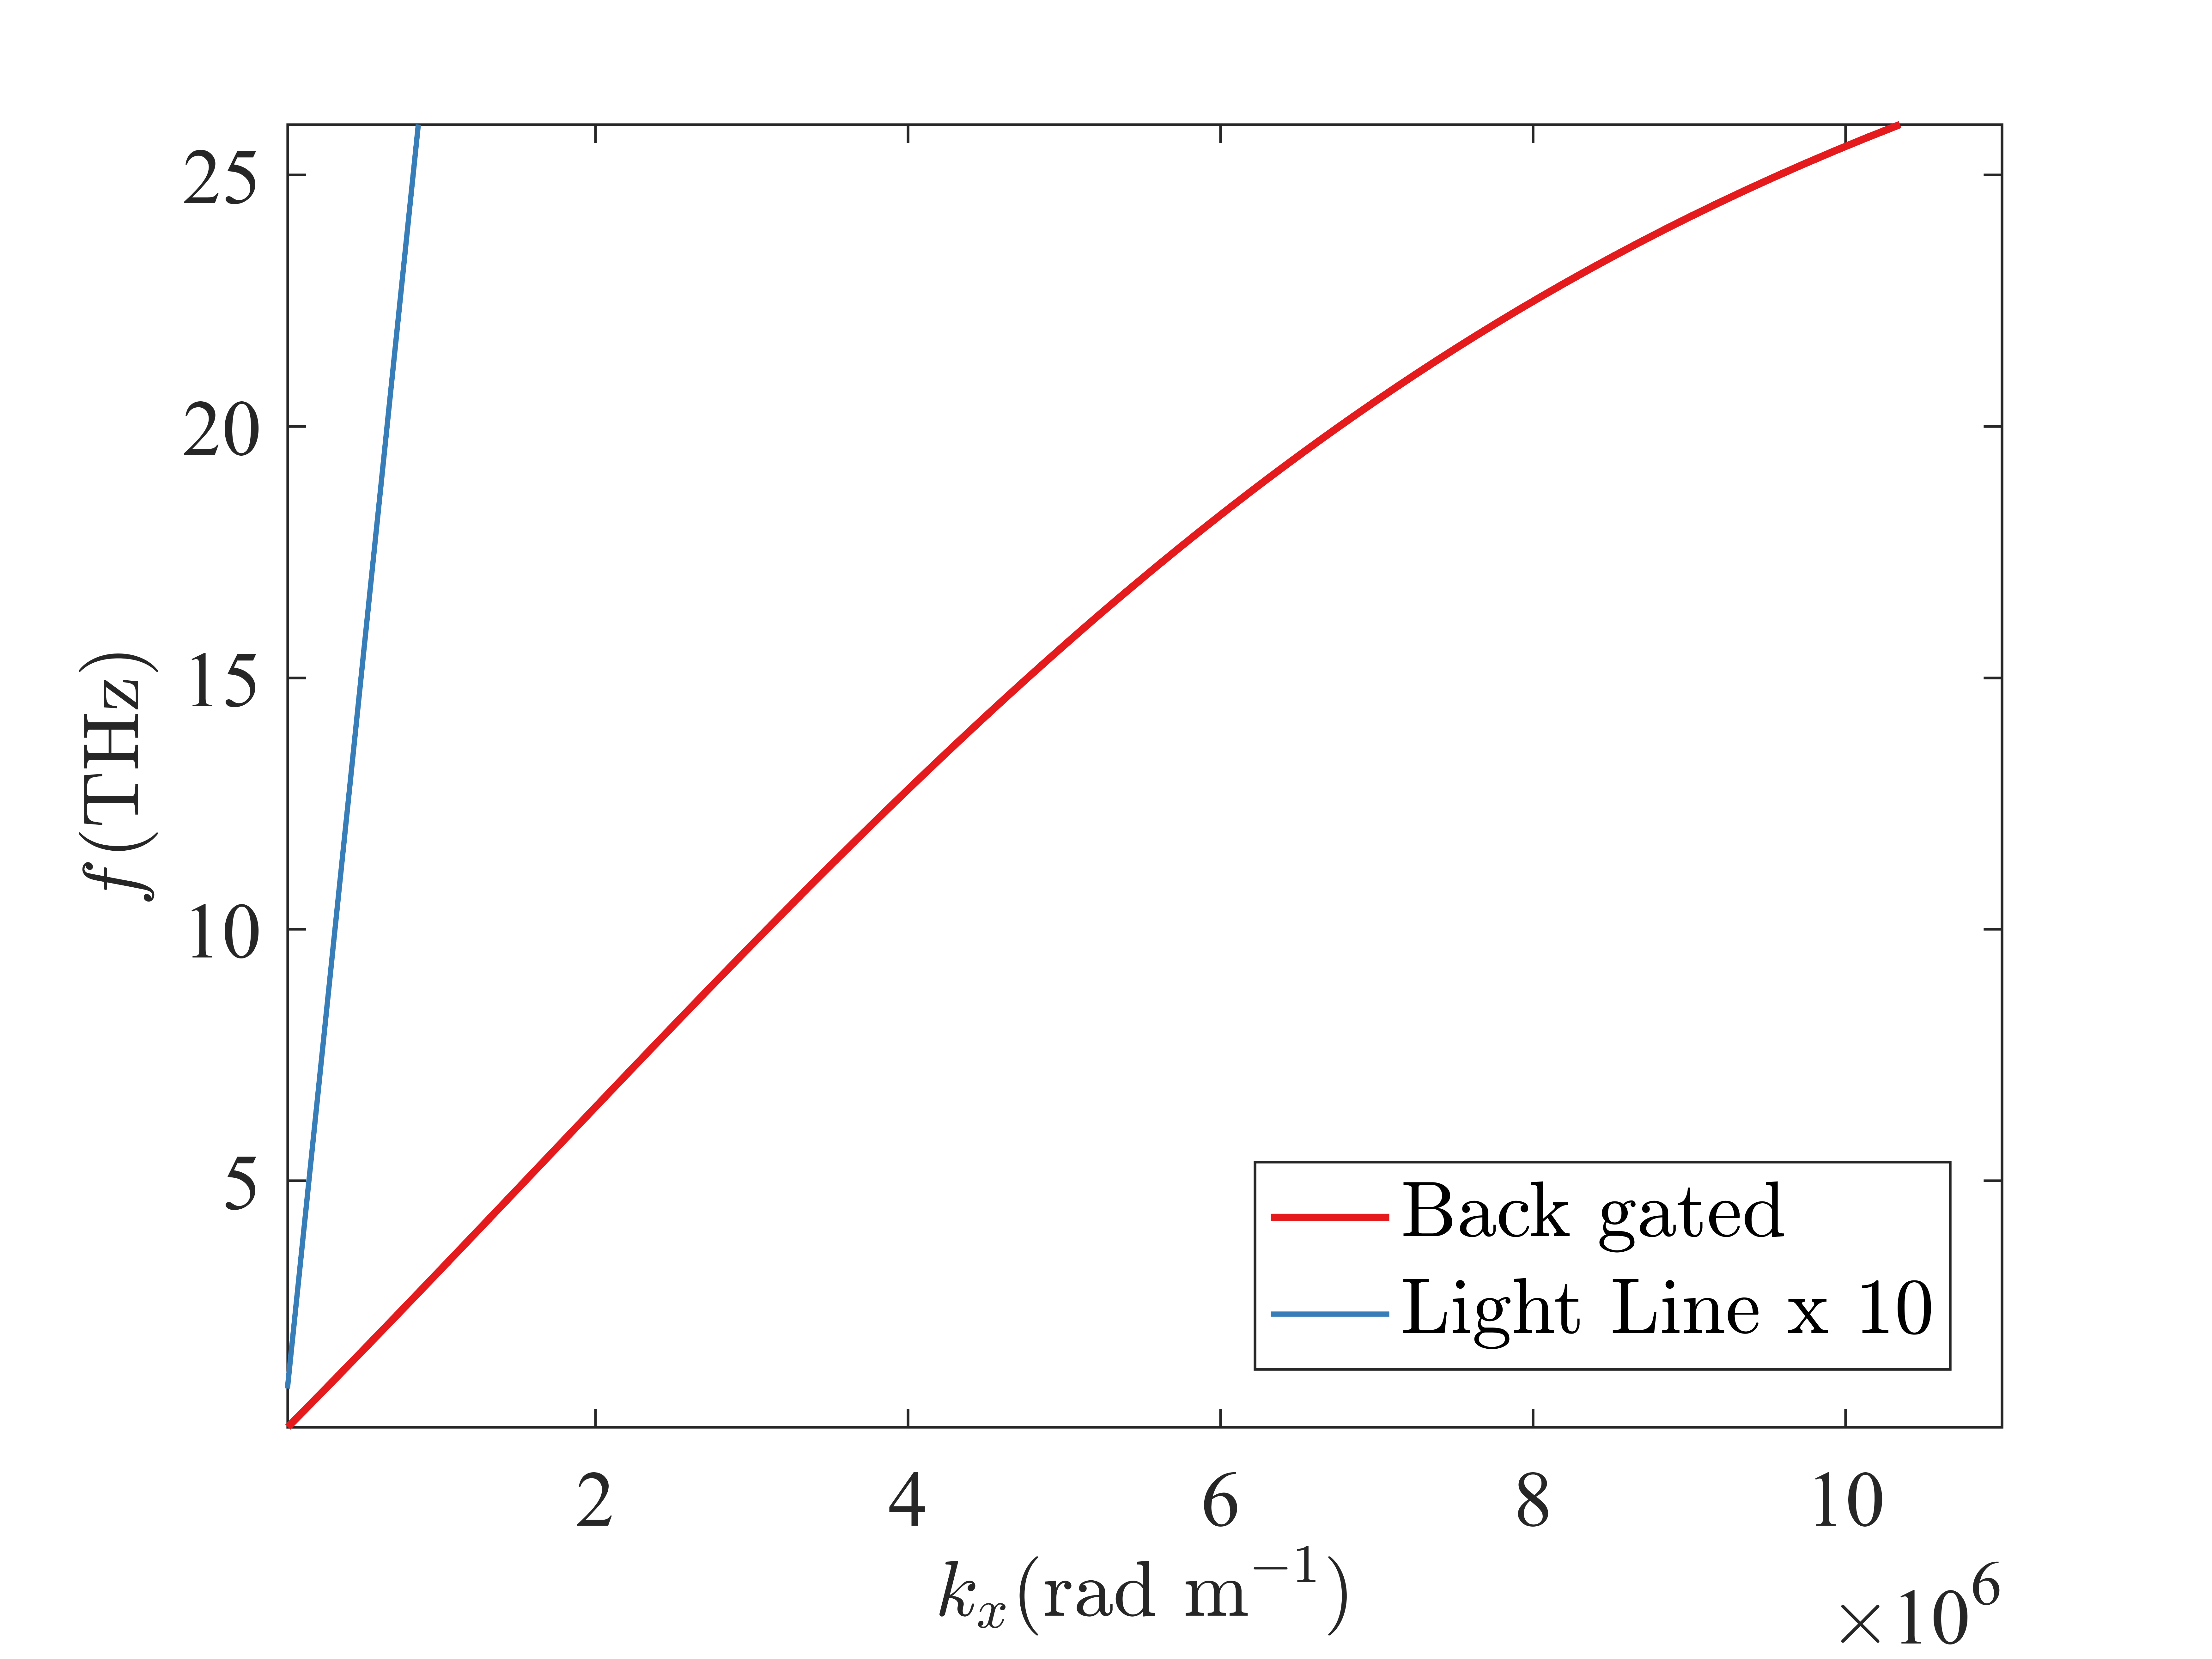
\includegraphics[height = 2.4in]{gated_disp.tikz}
  \label{fig:gated_hf_lt}}
  \subfloat[]{\includegraphics[height = 2.4in]{backgated_disp.tikz}
  \label{fig:backgated_hf_lt}} \\
  \subfloat[]{\includegraphics[height = 2.4in]{ungated_disp.tikz}
  \label{fig:ungated_hf_lt}}
  \caption{Dispersion Curves plotted for a GaN/AlGaN heterostructure with $N_s = \SI{5e13}{\cm^{-2}}$ at \SI{3}{\kelvin} (a) Gated (b) Backgated (c) Ungated}
  \label{fig:dispersion_hif_lowT}
\end{figure}
%

To observe the effect of temperature, we now plot the dispersion curves at room temperature ($T = \SI{295}{\kelvin}$) which corresponds to a scattering time, $\tau$ of $\SI{114}{\fs}$.
% %
\begin{figure}[!htbp]
  \centering
  \subfloat[]{\includegraphics[height = 2.4in]{gated_disp_lossy.tikz}
  \label{fig:gated_hf_ht}}
  \subfloat[]{\includegraphics[height = 2.4in]{backgated_disp_lossy.tikz}
  \label{fig:backgated_hf_ht}} \\
  \subfloat[]{\includegraphics[height = 2.4in]{ungated_disp_lossy.tikz}
  \label{fig:ungated_hf_ht}}
  \caption{Dispersion Curves plotted for a GaN/AlGaN heterostructure with $N_s = \SI{5e13}{\cm^{-2}}$ at \SI{295}{\kelvin} (a) Gated (b) Backgated (c) Ungated}
  \label{fig:dispersion_hif_hiT}
\end{figure}
%

The conducting layer in the gated and back-gated cases depicts the gate terminal which is voltage biased in a normal transistor operation. By varying the voltage, we can subsequently modify the electron density in the 2DEG channel. In Figs. \ref{fig:dispersion_lof_lowT} and \ref{fig:dispersion_lof_hiT}, the dispersion curves of gated and backgated structures are plotted for $N_s = \SI{1e12}{\cm^{-2}}$ at \SI{3}{} and \SI{295}{\kelvin} respectively.
% % %
\begin{figure}[!htbp]
  \begin{center}
  \subfloat[]{\includegraphics[height=2.8in]{gated_disp_low.tikz}
      \label{fig:gated_lf_lt}}
      \hfil
  \subfloat[]{\includegraphics[height=2.8in]{backgated_disp_low.tikz}
  \label{fig:backgated_lf_lt}}
  \caption{Dispersion Curves plotted for a GaN/AlGaN heterostructure with $N_s = \SI{1e12}{\cm^{-2}}$ at \SI{3}{\kelvin} (a) Gated (b) Backgated}
  \label{fig:dispersion_lof_lowT}
  \end{center}
\end{figure}
%

\begin{figure}[!htbp]
  \begin{center}
  \subfloat[]{\includegraphics[height=2.8in]{gated_disp_lossy_low.tikz}
      \label{fig:gated_lf_ht}}
      \hfil
  \subfloat[]{\includegraphics[height=2.8in]{backgated_disp_lossy_low.tikz}
  \label{fig:backgated_lf_ht}}
  \caption{Dispersion Curves plotted for a GaN/AlGaN heterostructure with $N_s = \SI{1e12}{\cm^{-2}}$ at \SI{295}{\kelvin} (a) Gated (b) Backgated}
  \label{fig:dispersion_lof_hiT}
  \end{center}
\end{figure}

In the results shown, the lowest order $\text{TM}_0$ is plotted in all cases. By comparing the plots in Fig. \ref{fig:dispersion_hif_lowT} with the corresponding plots in Fig. \ref{fig:dispersion_hif_lowT}, it is apparent that by increasing the temperature from liquid helium state tot room temperature, loss expressed in terms of the imaginary part of the propagation constant is introduced. The imaginary part and the light line are enhanced for illustration.

The propagation constant belonging to the gated region exhibits a linear relationship \cite{Sydoruk2015,Ando1982} as shown in Figs. \ref{fig:gated_hf_lt} and \ref{fig:gated_hf_ht}. Whereas a parabolic type dispersion curve is observed for the ungated region in Figs. \ref{fig:ungated_hf_lt} and \ref{fig:ungated_hf_ht}. For the backgated structure, the plot is initially linear for lower frequencies, followed by a parabolic region. The behavior is shown in Figs. \ref{fig:backgated_hf_lt} and
\ref{fig:backgated_hf_ht}. Such a dispersion is generally attributed to surface plasmon polaritons existing at a dielectric-metal interface \cite{Yoon2014}.

Figures \ref{fig:dispersion_lof_lowT} and \ref{fig:dispersion_lof_hiT} show the plots of gated and backgated dispersion curves in which the 2DEG region is tuned to a lower electron concentration of $N_s = \SI{1e12}{\cm^{-2}}$. Reduction of $N_s$ by more than an order of magnitude results in a marked increase of the propagation constant \cite{Sydoruk2015a}.
%%%%%%%%%%%%%%%
%%%%%%%%%%%%%%%
%%%%%%%%%%%%%%%
\section{Conclusion}
%
In this chapter, the dispersion relation of various configurations of a GaN/AlGaN heterostructure is solved. The dispersion curves computed clearly show that the propagation constant in the 2DEG region, which is embedded in the multilayer, is much larger than free-space wavenumber. This translates to the ability to support subwavelength phenomenon. The effect of temperature on the  associated loss is also observed.

%%%%%%%%%%%%%%%
%%%%%%%%%%%%%%%
%%%%%%%%%%%%%%%
\clearpage % Force Bibliography to the end of document on a new page.
% If using biber
% \printbibliography
% \addbibresource{zubairy}
% else bibtex
\bibliography{citations}
\bibliographystyle{ieeetran}

\end{document}
